% Template: hình bình hành ABCD với hai đường chéo AC, BD cắt nhau tại O.
% A, B đặt tự do; D = A + vector tịnh tiến; C = B + cùng vector đó.
\documentclass[border=5pt]{standalone}
\usepackage{tikz}
\usetikzlibrary{calc}
\begin{document}
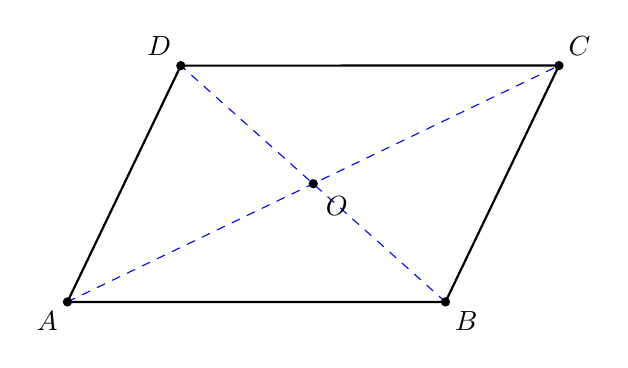
\begin{tikzpicture}[scale=1.2, line cap=round, line join=round]
  \coordinate (A) at (0,0);
  \coordinate (B) at (4,0);
  % vector AD
  \coordinate (D) at (1.2,2.5);
  % C = B + AD = A + AB + AD
  \coordinate (C) at ($(B)+(D)-(A)$);

  % Tâm O = giao của AC và BD = trung điểm AC
  \coordinate (O) at ($(A)!0.5!(C)$);

  % Cạnh
  \draw[thick] (A) -- (B) -- (C) -- (D) -- cycle;

  % Đường chéo
  \draw[blue, dashed] (A) -- (C);
  \draw[blue, dashed] (B) -- (D);

  % Chấm điểm
  \foreach \p in {A,B,C,D,O} \fill (\p) circle (1.4pt);

  % Nhãn
  \node[below left] at (A) {$A$};
  \node[below right] at (B) {$B$};
  \node[above right] at (C) {$C$};
  \node[above left] at (D) {$D$};
  \node[below right=1pt] at (O) {$O$};
\end{tikzpicture}
\end{document}
